%\documentclass[rnd]{mas_proposal}
\documentclass[thesis]{mas_proposal}

\usepackage[utf8]{inputenc}
\usepackage{amsmath}
\usepackage{amsfonts}
\usepackage{amssymb}
\usepackage{graphicx}
\usepackage{booktabs}

\usepackage{lipsum}
\usepackage{array}
\usepackage{makecell}

\renewcommand\theadalign{bc}
\renewcommand\theadfont{\bfseries}
\renewcommand\theadgape{\Gape[4pt]}
\renewcommand\cellgape{\Gape[4pt]}



\usepackage{xcolor}
\usepackage{listings}
\usepackage{caption}
\DeclareCaptionFont{white}{\color{white}}
\DeclareCaptionFormat{listing}{%
	\parbox{\textwidth}{\colorbox{gray}{\parbox{\textwidth}{#1#2#3}}\vskip-4pt}}
\captionsetup[lstlisting]{format=listing,labelfont=white,textfont=white}
\lstset{frame=lrb,xleftmargin=\fboxsep,xrightmargin=-\fboxsep}

\lstset{
	% numbers=left,
	breaklines=true,
	% backgroundcolor=\color{light-gray},
	tabsize=4,
	% basicstyle=\ttfamily,
	literate={\ \ }{{\ }}1	
}

\title{Compliant Manipulation with Task Specification and Reinforcement Learning}
\author{Abhishek Padalkar}
\supervisors{Prof. Dr. Paul G. Pl\"{o}ger\\Prof. Dr.-Ing. Gerhard K. Kraetzschmar \\Sven Schneider}
\date{\today}

% \thirdpartylogo{path/to/your/image}

\begin{document}

\maketitle

\pagestyle{plain}

\chapter{Introduction}
Most of the real world robotic manipulation tasks present the need for compliant manipulation, where robot needs to respond to the contact forces while executing the task. Classical planning and control algorithms fail to perform satisfactorily due to the lack of precise models of contact forces and high computational complexity. Various approaches have been proposed to learn compliant manipulation skills with help of Reinforcement Learning (RL). RL, in theory, is very promising when it comes to learn intelligent behaviors in complex environment with high dimensions. But it requires high number of interactions with environment. In model free reinforcement learning, a agent learns the skills by exploring the environment and adopting the parameters which governs the trajectory of the agent in the environment. Learning all the parameters of the policy can be computationally very expensive and might require large number of interactions with the environment. Application of RL to robotics is limited by above reason because large number trials causes wear and tear in mechanical parts and even damage to robot and the environment apart from being time consuming. Model based RL provide the solution to the problem of required high number of interactions with the environment by modeling some part of environment and motions policy. 

On the other hand, task specification approaches, proposed in \cite{leidner2017cognitive,mason1981compliance,bruyninckx1996specification} rely on instantaneous task specification in task frame where constraint on motion are specified in each direction. Such approaches are more practical because of their deterministic nature which can be used for ensuring safe robot operation. But some parameters used in task specification need to be tuned manually which is tedious task and require number of human interventions. Moreover, sometimes, the task is too complex to be specified fully using task specification. 

Nemec et al. in \cite{nemec2017door} propose a control algorithm by joining reinforcement learning with intelligent control which learns force policy to open door on top of the specified motion for unlatching and opening door operation.
We propose to extend above mentioned work by using task specification approach and using reinforcement learning for searching parameters good enough for executing the task maximizing given reward function. Our approach combines the features from model based manipulation solutions and reinforcement learning. We propose to bring together the feature of deterministic solution from model based control solutions and self learning capability from reinforcement learning in one solution.  


\section{Problem Statement}
\begin{itemize}
	\item To develop a learning based approach for achieving compliant manipulation that allows to exploit partial/incomplete models
	of the task and the environment.
	\item We plan to solve above problem by dividing the problem into two subproblems:
	\begin{itemize}
		\item Model the available knowledge about task and environment using existing task specification framework.
		\item Use reinforcement learning for parameter search or policy search which account for the unmodeled knowledge os the task and environment.
	\end{itemize}
    \item We will demonstrate our approach by learning a demo tasks of 
    \begin{itemize}
    	\item Opening door,
    	\item Wiping table,
    	\item Cutting vegetables.
    \end{itemize}
\end{itemize}


\chapter{Related Work}
\section{Task specification}
In industrial settings, task are usually specified in the form of sequence of primitives \cite{leidner2017cognitive}. These primitives mostly contain point-to-point motion, motion to some default configuration and basic curves. For example, following script taken from FRI interface examples shows the example motion primitives as shown in listing \ref{KRL-sample}. Though this kind of task specification works in controlled industrial environment, it leaves very little scope for external sensory feedback and the task needs to specified in terms of positional goals.

\begin{lstlisting}[label=KRL-sample,caption=KUKA Robot Language code]
INI
PTP HOME ; go to HOME joint configuration
LIN P1      ; linear motion to point P1
LIN P2	 ; linear motion to point P2
\end{lstlisting}

In \cite{leidner2017cognitive}, Leidner presented a representation in the form of action templates describing robot action using symbolic representations and geometric process model as shown in listing \ref{a-template}.  Symbolic representation of the task in PDDL allows classical planners to consider the action in the high level abstract task plan and geometric representation of the task specifies the sequence of low level movement sequences needed to complete the action. Here, geometric representation only specifies discrete motion primitives and not the parametric representation of the motion primitives. Actual parameterization and control is left to low level control module.   

\begin{lstlisting}[label=a-template,caption=Action Template: \_object.pick]
I Symbolic Representation 

'''
(:action _object.pick: 
:parameters (?o - _object ?m - _manipulator ?s - _surface) 
:precondition (and(free ?m) (on ?o ?s)) 
:effect (and(bound ?o ?m) (not(free ?m)) (not(on ?o ?s)))
) 
''' 

II Geometric Representation

def pick(self, manipulator, surface):
''' approach, grasp, and lift an object from a surface '''

graspset = odb.get_property(self.type, 'graspset', manipulator) 
for grasp_candidate in graspset: 
if grasp_candidate in self.history: 
continue
self.history.append(candidate) 
grasp = grasp_candidate 
break

if grasp is None: 
raise RuntimeError('no more alternatives')
else: 
self.grasp = grasp
operations = [
('move_hand', manipulator, g.approach_grasp), 
('plan_to_frame', manipulator, g.approach_frame, self.frame), ('plan_to_frame', manipulator, g.grasp_frame, self.frame), 
('bind', manipulator, self.name), 
('move_hand', manipulator, g.pre_grasp), 
('move_hand', manipulator, g.grasp), 
('move_straight', manipulator, txyz(0, 0, 0.1))
] 
return operations
\end{lstlisting}

In \cite{mason1981compliance}, Mason et. al. presented the idea behind \textit{Task Frame Formalization - TFF} for representing compliant task. Using hybrid control, various control modes are assigned to each axis of the \textit{task frame} or \textit{compliance frame}\cite{nagele2018prototype}. Listing \ref{tff} shows Open Door task taken from \cite{bruyninckx1996specification}. This framework doesn't consider the specification of task or motion quality related parameters like velocity damping or instantaneous sensory inputs. It also specify action to be executed \textit{compliantly} but does not specify the how? 

\begin{lstlisting}[label=tff,caption=Task Specification using TFF: Open Door]
move compliantly {
	with task frame directions
	xt: force 0 N
	yt: force 0 N
	zt: velocity v mm/sec
	axt: force 0 Nmm
	ayt: force 0 Nmm
	azt: force 0 Nmm
} until distance > d mm 
\end{lstlisting}


iTaSC developed in \cite{DeSchutter-ijrr2007, DecreBruyninckxDeSchutter2013, decre09}, synthesizes control inputs based on provided task space constraints. It formulates a optimization problem considering provided constraints in the environment. In case of conflicting constraints, constraints are weighted in the optimization problem. 

\chapter{Reinforcement Learning}

Ideally, using reinforcement learning, an agent can find an optimal or near optimal behavior by interacting with the environment. Instead of providing a detailed engineered solution, a reward function provides the feedback on the task which enables agent to learn a optimal solution. Based on use of prior knowledge, reinforcement learning approaches are categorized in two categories namely Model based and Model free reinforcement learning.  

\section{Model Free Reinforcement Learning}

In model free reinforcement learning, no model of transition dynamics exist, hence optimal actions are derived by trial and error\cite{polydoros2017survey}. Learning all the parameters of the policy can be computationally very expensive and might require large number of interactions with the environment. Moreover, traditional RL methods utilize discrete state/action representation, which results into huge state-action space\cite{nemec2017door}. Application of model free reinforcement learning to robotics is limited by above reason, as large number of trials causes wear and tear in mechanical parts and even damage to robot and the environment apart from being time consuming.

\section{Model Based Reinforcement Learning} \label{mod-RL}
In model based  reinforcement learning, the model of transition dynamics exists. This transition model is used for deriving rewards and optimal actions. Optimal actions are derived using internal simulations reducing the number of interactions needed. This optimal policy is then executed in the environment. But this approach too heavily suffers from the accuracy of the transition dynamics model. Value function based RL methods learn the model by interacting with the envionment and then deriving the control policy using methods like \textit{Differential Dynamic Programming, Temporal Difference Learning, Policy Iteration, Monte Carlo and Value Iteration}\cite{polydoros2017survey}. Some of the approaches implemented in robotics use reinforcement learning for learning direct control policy, rather than learning model and then deriving the policy\cite{polydoros2017survey}. Polydoros et al. give comprehensive survey on model based RL in \cite{polydoros2017survey}. 

Nemec et al. use reinforcement learning for learning force control policy for opening door\cite{nemec2017door}. They take into account the constraints on the door motion and cosed kinematic chain resulting from a firm grasp of robot hand on the door handle. While opening the door in such configuration, high internal forces are generated in the direction where motion is not possible. They use this knowledge to learn a compliant force control policy. Our approach is motivated by this work of Nemec et al.\cite{nemec2017door}. We try to formalize constraints in terms of already existing task specification methods, which can be generalized to more number of compliant manipulation tasks. 

\section{Door Opening Task}

Opening door is one the most important task for service and rescue robots. Number of studies have been conducted to investigate this challenging problem using different techniques. Number of approaches rely on detail geometric modeling of the door and analytical trajectory generation. Nagatani et.al. \cite{nagatani1995experiment} presented an early approach for opening door by modeling the geometry of the door and then synthesizing trajectory to open door by considering geometrical constraints. To cope with the errors in position control of the early days manipulator used in the experiment, they used a force torque sensor module to achieve compliance with the environment. But this approach highly relies on correct geometric model and accurate execution of designed trajectories.

Approaches presented in \cite{levihn2014using,karayiannidis2012adaptive,niemeyer1997simple} use adaptive control algorithms which synthesize the motion by identifying the environmental constraints. In \cite{karayiannidis2012adaptive}, authors proposed to find the radial direction based on force and torque readings. Door is opened by applying velocity in radial direction. This method is prone to failure in case of uncertain grasp position. Also it considers only the case where door is already unlatched. 

Some of the methods for door opening motor primitives like Dynamic motion primitives for generating trajectories for opening door. Disadvantage of these approaches is that we need to know the goal pose to generate trajectory hence it confines the condition of completing the task to achieving a goal pose. 

\section{Vegetables Cutting Task}
Vegetable cutting task in an interesting problem for robot manipulation considering the complexity of contact forces. Different vegetables requires different cutting forces. Also force profile changes as we cut through the vegetables, e.g. tomato requires much less force once we cut through the skin. Such a complicated force interactions are very hard to model and specified in the task specification. Reinforcement learning provides the solution by allowing robots to learn force control policy over time or phase of the cutting task. This task was chosen for demonstration because of its complex contact force profile. Moreover the task itself does not need any external sensors other than force torque sensors to for estimating rewards and completion of the task.

In \cite{lioutikov2016learning}, Lioutikov et al. solved the task by learning Dynamic Motion Primitives, which is a trajectory control policy. Authors does not consider the problem as compliant manipulation problem hence contact forces are not taken into account. Task is solved just by performing Cartesian trajectory, and hence requiring multiple attempts to cut through the vegetable. 


\chapter{Proposed Solution}

We plan to solve a compliant manipulation task by providing a incomplete task specification and using Reinforcement Learning to determine un-modeled components in task specification. We propose to create a framework based on task specification and model based reinforcement learning to solve the problem of compliant manipulation for given task in deterministic manner with fewer number of interactions with environment.

\section{Composition}

\begin{figure}[!h]
	\center{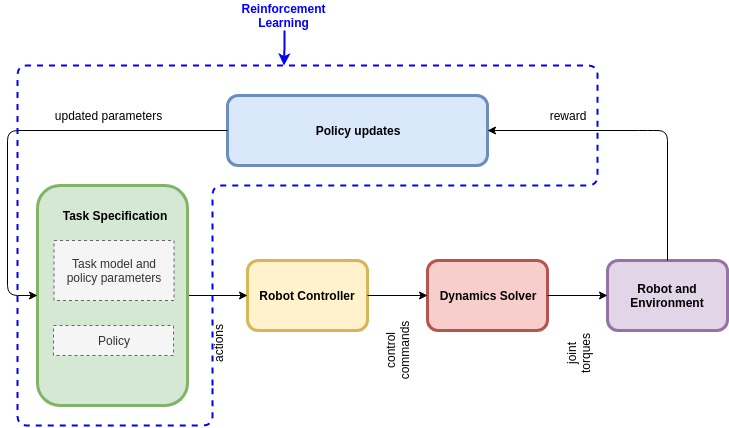
\includegraphics[width=\textwidth]
		{images/composition.png}}
	\caption{\label{fig:composition} Composition}
\end{figure}
Above figure shows the composition of the proposed solution.

\section{Task Specification}
We propose to use approach given by Mason et al.\cite{mason1981compliance}, with further modification considering limitation on robot and environment. These parameters will also be used for ensuring quality of the task. e.g. smoothness in opening door. Also we introduce force and velocities as functions of robot and environmental parameters and phase of the task. 
\newpage
\textbf{Examples of task specification:} 
\begin{lstlisting}[label=open_door_ts,caption=Task specification for opening door]
open_door
{
	with task frame directions
	xt: force 0 N
	yt: force 0 N
	zt: force f(environment, robot, task) N
	axt: force 0 Nmm
	ayt: force 0 Nmm
	azt: force 0 Nmm
	max_acc = a_max m/ss
	max_dec = a_dec m/ss
}until(g(...))

\end{lstlisting}

In above mentioned door opening task, task is represented in door frame where z-axis is perpendicular to door frame. Here, instead of specifying force in the z-direction, a constant velocity can also be specified for simplicity. But such specification can result in oscillations in case of self closing doors where initially huge amount force is required to move the door. It can be a huge problem especially when velocity control loop is running at low frequency. Parameters max\_acc and max\_dec ensure safe operation of the robot as well as quality of task.


In vegetable cutting task stated in Listing \ref{cut_vegies}, task is represented in chopping board frame such that z-axis is perpendicular to the chopping board and x-axis is in cutting direction. In this task, velocity in x-axis and force in z-axis are not easy to be modeled or parameterized. Here both of these entities can be represented by and time parameterized policy. Moreover velocity can be learned from demonstrations using methods like Dynamic Motions Primitives\cite{lioutikov2016learning}. 

\newpage
\begin{lstlisting}[label=cut_vegies,caption=Task specification for cutting vegetables]

cut_vegetables
{
	with task frame directions
	xt: velocity v(t) m/s
	yt: force 0 N
	zt: force f(environment, robot, task, xt) N
	axt: force 0 Nmm
	ayt: force 0 Nmm
	azt: force 0 Nmm
	max_acc = a_max m/ss
	max_dec = a_dec m/ss
}until(g(...))

\end{lstlisting}



\section{Reinforcement Learning Algorithm}

As already discussed, \begin{enumerate}
	\item Task specification approaches are reliable but they need manual tuning of many parameters
	\item Sometimes force interactions in compliant manipulation tasks are so complex that parameterization of task and force control policy is not possible. 
\end{enumerate}
Both of the above mentioned problems can be tackled by reinforcement learning. In first case, where the parameterization is possible, model based RL methods can be used for searching near optimal model parameters. Then policy can be derived by methods mentioned in section \ref{mod-RL} and in \cite{polydoros2017survey}. It is even possible to specify a engineered policy which uses the learned parameters.

Tasks where policy parameterization is not possible, model based RL can be used directly to learn a generic parameterized policy by using methods like \textit{Gradient-based approaches, Sampling based approaches, Information theory methods, Evolutionary computation, etc}\cite{polydoros2017survey}. 

In our case, we plan to represent control policy in terms of weighted Gaussian functions similar as in \cite{nemec2017door}. We plan to use Policy Improvement with Path Integral ($\text{PI}^{2}$) algorithm\cite{theodorou2010learning} for optimizing the policy parameters. ($\text{PI}^{2}$) is a sampling based algorithm which uses zero mean Gaussian noise to generate new parameters.    

\section{Robot Controller}

We propose to use robot specific impedance controller for controlling the robot. For KUKA LWR robot this controller is already provided by the manufacturer which is stated by following equation taken from \cite{schreiber2010fast}, an official documentation for KUKA Fast Research Interface.

\begin{equation}
\tau_{cmd} = J^{T}(K_{c}(x_{FRI} - x_{msr}) + D(d_{c}) + F_{FRI}) + f_{dynamics}(q, \dot{q}, \ddot{q})
\end{equation}

Where,
$\tau_{cmd}$ is commanded joint torque, $J$ is jacobian of manipulator, $K_{c}$ is spring constant or stiffness constant, $x_{FRI}$ is commanded Cartesian position, $x_{msr}$ is current measured Cartesian position, $d_{c}$ is Cartesian normalized damping parameter, $F_{FRI}$ is commanded Cartesian force vector. The terms for the damping design $D(d_{c})$ and the dynamic model $f_{dynamics}(q, \dot{q}, \ddot{q})$ are taken care of in the KUKA motion
kernel.   

For manipulators which don't have internal torque controllers, but are equipped with the wrist force-torque sensors, impedance control can be achieved by a linear PID feedback controller which in turn controls velocity of end effector to control force and torque at end effector. Here the feedback is force and torque measurements by wrist force torque sensor. Such controller can be given by equation below:
\begin{align}
	v =& P \cdot f_{e} + I \cdot \int f_{e} + D \cdot \dot{f_{e}} \\
	f_{e} =& f_{desired} - f_{measured}
\end{align}   
Where, $v$ is velocity vector of end effector.
\chapter{Project Plan}
Project plan for this master thesis is as follows:
\section{Work Packages and Milestones}

\begin{tabular}{|c|c|c|}

	\hline
	\multicolumn{2}{|c|}{\thead{Work Packages}} & \thead{Targeted date} \\
	\hline
	WP01 & Literature search & 10-05-2019 \\
	WP02 & Analysis of state of the art &  \\
	\textit{MS01} & \textit{Documentation of the state of the art} &  \\
	\hline 
	WP03 & Modeling demo tasks using task specification approach &  20-06-2019\\ 
	WP04 & Design and implementation of the robot controller &   \\
	\textit{MS02} & \textit{Implementing task specification approach for door opening} &  \\
	\hline
	WP05 & Integrating RL algorithm in task specification & 30-07-2019 \\ 
	WP06 & Design and implementation of RL algorithm &   \\
	\textit{MS03} & \makecell{\textit{Implementing task specification approach} \\ \textit{with RL for door opening task}} &  \\
	\hline
	WP05 & Extending implemented solution for vegetable cutting task & 10-09-2019 \\ 
	WP06 & Experimental evaluation of implemented algorithms &  \\
	\textit{MS03} & \makecell{\textit{Implementing task specification approach with} \\ \textit{RL for cutting vegetable task}} &  \\
	\hline
\end{tabular}


\section{Project Schedule}



\section{Deliverables}
Deliverables of this project are as follows: 
\subsection{Minimum Viable}

\begin{itemize}
    \item Literature survey and analysis of the state of the art.
    \item Design and implementation of task specification framework with reinforcement learning.
    \item Demonstration of task specification framework for door opening task without using reinforcement learning.
\end{itemize}

\subsection{Expected}
\begin{itemize}
    \item Demonstration of task specification framework with reinforcement learning for door opening task.
\end{itemize}

\subsection{Desired}
\begin{itemize}
	\item Extending proposed approach for cutting vegetable task.
    \item Demonstration of task specification framework with reinforcement learning for vegetable cutting task.
\end{itemize}


\nocite{*}

\bibliographystyle{plainnat} % Use the plainnat bibliography style
\bibliography{bibliography.bib} % Use the bibliography.bib file as the source of references




\end{document}
